\documentclass[12pt, a4paper
,openany
]{Thesis} % Paper size, default font size and one-sided paper
%% Change format for two-sided printing
\newcounter{print}
\setcounter{print}{0}    
    % comment out line 2 and give argument 1 for print layout
    % uncomment line 2 and give argument 0 for digital layout
    


\def\dissertationTitleX{SSL Automation Tool\\For\\StartMySafari Innovations Private Limited (smsipl)}
\def\dissertationTitle{SSL Automation Tool}
\def\degree{Master of Computer Application}
\def\ttitle{Project Report}
\def\authornames{Dipak Nivrutti Rathod}
\def\authorrollno{MCD004036}
\def\deptname{Department of Management Science}
\def\univname{Dr. Babasaheb Ambedkar Marathwada University, Chhatrapati Sambhajinagar}

\usepackage{sectsty}
\chapterfont{\centering}
\usepackage{emptypage}
\usepackage{nicefrac}
\usepackage[inkscapeformat=png]{svg}
% \usepackage[none]{hyphenat}
\tolerance=1
\emergencystretch=\maxdimen
\hyphenpenalty=10000
\hbadness=10000

% Custom border for title and certificate page
\usepackage{fancybox}
\newcommand{\thickborder}[1]{%
  \setlength{\fboxrule}{2pt}%
  \setlength{\fboxsep}{8pt}%
  \fbox{#1}%
}

% \usepackage[resetlabels,labeled]{multibib}

\usepackage[utf8]{inputenc}
\usepackage{wrapfig}
\usepackage{lscape}
\usepackage{rotating}
\usepackage{graphicx}
\usepackage{caption}
\usepackage{amsmath, nccmath}
\usepackage{comment}
\usepackage{afterpage}
\usepackage{multirow}
\usepackage{multicol}
\usepackage{cleveref}
\usepackage{rotating}
% \usepackage[font=small]{caption}
% \captionsetup{compatibility=false}
% \usepackage{subcaption}
% \usepackage{subfig}
\usepackage{makecell}
\usepackage{booktabs}
\usepackage{multirow}
\usepackage{lscape}
\usepackage{longtable}
\usepackage{placeins}
\usepackage{adjustbox}
\usepackage{arydshln} % dashed midline
\usepackage{ragged2e}
\usepackage{lipsum}
\usepackage{mathtools} % To use box inside an aligned environment
\usepackage{enumitem} % for roman letter lists
% \usepackage{subfig}
\newcommand\myemptypage{
    \newpage
    \null
    \pagestyle{empty}
    % \addtocounter{page}{-1}
    \newpage
    \pagestyle{plain}
    }
%\usepackage[width=14cm, left=3cm]{geometry}

% prints author names as small caps


%\usepackage{subcaption} %incompatible with subfig
\graphicspath{{Pictures/}} % Specifies the directory where pictures are stored
% \usepackage[authoryear]{natbib}
%\usepackage[square, numbers]{natbib} % Use the natbib reference package - read up on this to edit the reference style; if you want text (e.g. Smith et al., 2012) for the in-text references (instead of numbers), remove 'numbers' v
%\bibliographystyle{abbrvnat}
%\setcitestyle{authoryear,open={((},close={))}}
\hypersetup{urlcolor=blue, colorlinks=true} % Colors hyperlinks in blue - change to black if annoyingv`	
\title{\ttitle} % Defines the thesis title - don't touch this




%%%% New added


\usepackage{tikz}
\usetikzlibrary{shapes.geometric, arrows}

% Defining Tickz Style
\tikzstyle{startstop} = [rectangle, rounded corners, minimum width=3cm, minimum height=1cm, text centered, text width = 10cm, draw=black, fill=white]

% \tikzstyle{startstop1} = [rectangle, rounded corners, minimum width=3cm, minimum height=1cm, text centered, draw=black, fill=white, text width = 10cm]

% \tikzstyle{io} = [trapezium, trapezium left angle=70, trapezium right angle=110, minimum width=3cm, minimum height=1cm, text centered, text width = 4.5cm, draw=black, fill=blue!30]

\tikzstyle{process} = [rectangle, minimum width=3cm, minimum height=1cm, text centered, text width = 6cm, draw=black, fill=white, text width = 10cm]

% \tikzstyle{decision} = [diamond, minimum width=3cm, minimum height=1cm, text centered, draw=black, fill=green!30]

\tikzstyle{arrow} = [ultra thick,->,>=stealth, line width=0.7mm]

% Add calc library for positioning in borders
\usetikzlibrary{calc}





\usepackage[T1]{fontenc}

\usepackage{hyperref}

% Define a nice-looking page style with consistent headers and footers
\pagestyle{fancy}
\fancyhf{} % Clear all header and footer fields
\fancyhead[LE,RO]{\thepage} % Left on even pages, right on odd pages for page number
\fancyhead[RE]{\textit{\nouppercase{\leftmark}}} % Right on even pages chapter
\fancyhead[LO]{\textit{\nouppercase{\rightmark}}} % Left on odd pages section
\fancyfoot[C]{} % No footer
\renewcommand{\headrulewidth}{0.4pt} % Line thickness at the header
\renewcommand{\footrulewidth}{0pt} % No line at the footer
\fancypagestyle{plain}{%
  \fancyhf{} % Clear header and footer fields
  \fancyfoot[C]{\thepage} % Center-bottom page number on plain pages
  \renewcommand{\headrulewidth}{0pt} % No line at the header
  \renewcommand{\footrulewidth}{0pt} % No line at the footer
}

% Redefine chapter and section marks to be more consistent
\renewcommand{\chaptermark}[1]{\markboth{\chaptername\ \thechapter.\ #1}{}}
\renewcommand{\sectionmark}[1]{\markright{\thesection.\ #1}}

\begin{document}

% Add 2 blank pages at the beginning
\thispagestyle{empty}
\null
\newpage

\thispagestyle{empty}
\null
\newpage

% prints author names as small caps
% it is sometimes necessary in user documents to have access to such package-internal macros, and so the commands \makeatletter and \makeatother change the catcode 


\frontmatter % Use roman page numbering style (i, ii, iii, iv...) for the pre-content pages

\setstretch{1.6} % Line spacing of 1.6 (double line spacing)

% Define the page headers using the FancyHdr package and set up for one-sided printing
\fancyhead{} % Clears all page headers and footers
\fancyfoot{}
% \rhead{\thepage} % Sets the right side header to show the page number
% \lhead{} % Clears the left side page header
\fancyhead[LE,RO]{\thepage} % page at left on even and right on odd pages

\pagestyle{fancy} % Finally, use the "fancy" page style to implement the FancyHdr headers

\newcommand{\HRule}{\rule{\linewidth}{0.5mm}} % New command to make the lines in the title page

% PDF meta-data
\hypersetup{pdftitle={\ttitle}}
% \hypersetup{pdfsubject=\subjectname}
\hypersetup{pdfauthor=\authornames}
% \hypersetup{pdfkeywords=\keywordnames}




% --------------------------------------------------





%----------------------------------------------------------------------------------------
%	TITLE PAGE
%----------------------------------------------------------------------------------------
\begin{comment}
\begin{titlepage}
\begin{center}

\HRule \\[0.4cm] % Horizontal line
{\huge \bfseries \ttitle}\\[0.4cm] % Thesis title
\HRule \\[1.5cm] % Horizontal line
 
\large \textit{A thesis submitted in fulfillment of the requirements\\ for the degree of \degreename}\\[0.3cm] % University requirement text
\textit{by}\\[0.4cm]

%\href{http://home.iitk.ac.in/~saiwal}{\authornames}

\vfill
\graphicspath{ {./Figures/} }
\begin{figure}[hb]
  \centering
  \includegraphics[width=0.4\linewidth]{Images/redlogo.png}
\end{figure}

\DEPTNAME\\ % Research group name and department name
\textsc{ \UNIVNAME}\\[1.5cm] % University name
\large \today\\[2cm] % Date


\end{center}

\end{titlepage}
\end{comment}
%\begin{document}
%\begin{titlepage}


%\include{title1}
%\end{titlepage}
%\myemptypage
%\afterpage{\null\newpage}
%\include{blank_page_1}
%\newpage
%\newpage
%\newgeometry{centering,top = 2.54cm,bottom = 2.54cm,left = 2.54cm, right = 2.54cm, includeheadfoot}

\pagenumbering{gobble}% Remove page numbers (and reset to 1)
\thispagestyle{empty}
\singlespacing
\begin{titlepage}
% Simple frame around entire page content using the thicker border
\thickborder{%
\begin{minipage}{\dimexpr\textwidth-2\fboxsep-2\fboxrule\relax}
\vspace{0.5cm}

\vspace*{-2.0cm} % Move everything up even more
\begin{center}
    \centering
     
%=====================================================%
%---------------PROJECT REPORT TITLE-----------------%
%=====================================================%    
\definecolor{blue}{rgb}{0,0,1}
      
  {{\LARGE \textbf{PROJECT REPORT}\par}}
    \vspace{0.2cm}
  {{\LARGE \textbf{ON}\par}}
    \vspace{0.2cm}
  {{\LARGE \textbf{SSL Automation Tool}\par}}
    \vspace{0.2cm}
  {{\large \textbf{StartMySafari Innovations Private Limited (smsipl)}\par}}
    \vspace{0.7cm}
     
%=====================================================%
%---------------AUTHOR'S NAME-------------------------%
%=====================================================%

    {\large \textbf{Submitted by}\par}
    \vspace{0.2cm}
    {\large \textbf{\textcolor{blue}{Dipak Nivrutti Rathod}}\par}
    \vspace{0.1cm}
    {\large \textbf{Seat No: MCD004036}\par}
    \vspace{0.7cm}
    
%=====================================================%
%---------------Supervisor Name---------------------%
%=====================================================%    
    {{\large \textbf{UNDER THE GUIDANCE OF}}\par}
    \vspace{0.2cm}
    {\large \textbf{\textcolor{blue}{Dr. Kavari Lad}}\par}
    \vspace{0.7cm}

%=====================================================%
%---------------Partial Fulfillment---------------------%
%=====================================================%
    {In partial fulfilment for the award of the degree of \par}
    \vspace{0.2cm}
    {\large \textbf{MCA (Master of Computer Application)} \par}
    \vspace{0.7cm}

\vspace{0.2cm}
%=====================================================%
%---------------UNIVERSITY lOGO-----------------------%
%=====================================================%
\includegraphics[width=30mm]{Images/iitb_logo.png}
    \vspace{0.2cm}

    
%=====================================================%
%---------------DEPARTMENT'S NAME-------------------------%
%=====================================================%   
    {\large \textbf{Dr. Babasaheb Ambedkar Marathwada University, Chhatrapati Sambhajinagar}\par}
    \vspace{0.1cm}
    {\large Department of Management Science \par}
    \vspace{0.1cm}
%=====================================================%
%---------------DATE----------------------------------%
%=====================================================%
    {\large \textbf{2023-24}}

\end{center}
\vspace{0.5cm}
\end{minipage}%
}
\end{titlepage}
\pagenumbering{gobble}% Remove page numbers
\thispagestyle{empty}

% Simple frame around the content using thicker border
\thickborder{%
\begin{minipage}{\dimexpr\textwidth-2\fboxsep-2\fboxrule\relax}
\vspace{0.5cm}

\begin{center}
    % Header with both logos
    \begin{minipage}{0.12\textwidth}
        \includegraphics[width=\linewidth]{Images/iitb_logo.png}
    \end{minipage}
    \hfill
    \begin{minipage}{0.7\textwidth}
        \centering
        \large\textbf{Dr. Babasaheb Ambedkar Marathwada University,}\\
        \large\textbf{Chhatrapati Sambhajinagar}\\
        \normalsize\textbf{Department of Management Science}
    \end{minipage}
    \hfill
    \begin{minipage}{0.12\textwidth}
        \includegraphics[width=\linewidth]{Images/udms-logo.png}
    \end{minipage}
\end{center}

\vspace{0.2cm}
\noindent\rule{\linewidth}{1pt}
\vspace{1.5cm}

\begin{center}
    \textbf{\LARGE CERTIFICATE}
\end{center}

\vspace{1.2cm}

\begin{center}
\begin{minipage}{0.9\textwidth}
\large
This is to certify that \textbf{Dipak Nivrutti Rathod} (Seat No: \textbf{MCD004036}) has satisfactorily carried out the project work entitled \textbf{"SSL Automation Tool"} as per requirement of Department of Management Science, Dr. Babasaheb Ambedkar Marathwada University, Chhatrapati Sambhajinagar in the fulfillment of Master of Computer Application for the academic Year 2023-24.
\end{minipage}
\end{center}

\vspace{3cm}

% Guide and Director signatures on the same line
\noindent
\begin{minipage}{0.45\textwidth}
    \centering
    \rule{4cm}{0.4pt}\\
    \textbf{Dr. Kavari Lad}\\
    (Project Guide)
\end{minipage}
\hfill
\begin{minipage}{0.45\textwidth}
    \centering
    \rule{4cm}{0.4pt}\\
    \textbf{Prof. Abhijeet Shelke}\\
    (Director)
\end{minipage}

\vspace{1.5cm}
\begin{center}
\begin{minipage}{0.9\textwidth}
\begin{center}
\textbf{Date:} \underline{\hspace{3cm}} \hspace{2cm} \textbf{Place:} \underline{Chhatrapati Sambhajinagar}
\end{center}
\end{minipage}
\end{center}

% Push External Examiner to bottom of page
\vfill

% External Examiner at the footer
\begin{center}
\begin{minipage}{0.45\textwidth}
    \centering
    \rule{4cm}{0.4pt}\\
    \textbf{External Examiner}
\end{minipage}
\end{center}

\vspace{0.5cm}
\end{minipage}%
}

\clearpage  % Adding certificate page
% Acknowledgements

\addtocontents{toc}{} % Add a gap in the Contents, for aesthetics
\thispagestyle{empty}
\acknowledgements{

I would like to express my sincere gratitude to all those who contributed to the successful completion of this SSL Automation Tool project.

First and foremost, I extend my heartfelt thanks to \textbf{Dr. Kavari Lad}, my project guide, for his invaluable guidance, continuous support, and expert advice throughout the development of this project. His insights into modern web technologies and security practices were instrumental in shaping this work.

I am deeply grateful to \textbf{StartMySafari Innovations Private Limited (smsipl)} for providing the opportunity to work on this practical and industry-relevant project. The real-world exposure and access to modern development tools and technologies significantly enhanced my learning experience.

Special thanks to \textbf{Prof. Abhijeet Shelke}, Director, for his administrative support and for creating an environment conducive to learning and innovation.

I would like to acknowledge the faculty members of the Department of Management Science at \textbf{Dr. Babasaheb Ambedkar Marathwada University, Chhatrapati Sambhajinagar}, for their academic support and for providing the foundational knowledge that enabled me to undertake this project.

My appreciation extends to the open-source community, particularly the developers of React, Next.js, FastAPI, and Let's Encrypt, whose technologies formed the backbone of this SSL automation solution.

I am thankful to my colleagues and peers who provided feedback and suggestions during the development and testing phases of the project.

Finally, I express my gratitude to my family and friends for their constant encouragement and support throughout my academic journey.

This project has been an enriching experience that has significantly enhanced my understanding of web development, SSL certificate management, and modern software engineering practices.

\begin{flushleft}
    \textbf{\authornames}\\
    June 2025
\end{flushleft}
}
% 

% \newpage
% \myemptypage
\frontmatter
\setstretch{1.3}
\pagestyle{plain}
% %----------------------------------------------------------------------------------------
% %	DEDICATION
% %----------------------------------------------------------------------------------------
% %
% \setstretch{1.3} % Return the line spacing back to 1.3
% \addtocontents{toc}{\vspace{2em}} % Add a gap in the Contents, for aesthetics
% %

% %
% \dedicatory{\textit{Dedicated to my beloved parents.}} % Dedication text
% % \thispagestyle{empty}
% %

% % \myemptypage

% %----------------------------------------------------------------------------------------
% Approval page
%----------------------------------------------------------------------------------------
%\thispagestyle{empty} % Page style needs to be empty for this page
%
%\addtotoc{Approval}
%\addtocontents{toc}{}
%% \pagenumbering{roman}
%% \cfoot{\thepage}
%% \setcounter{page}{3}
%\vspace{-1in}
%\begin{center}
%{\LARGE  {\bf Dissertation Approval}}
%\end{center}
%\vspace*{0.1in} \noindent This project report entitled {\large \bf \dissertationTitle} by {\bf \large \authornames}, Roll No. \authorrollno, is submitted for the degree of  {\large \bf \degree} from Dr. Babasaheb Ambedkar Marathwada University, Chhatrapati Sambhajinagar.\\\\
%
%\vspace{2cm}
%
%  \hspace*{0.8cm}\ldots\ldots \ldots\ldots \ldots\ldots \ldots\ldots  \hspace{2in}  \ldots\ldots \ldots\ldots \ldots\ldots \ldots\ldots \\
%  \hspace*{0.4cm}\hspace*{0cm} Dr. Kavari Lad \hspace{1.85in} Prof. Abhijeet Shelke\\
%  \hspace*{0.8cm}\hspace*{0.9cm} (Project Guide) \hspace{2.8in} (Director)\\\\
%
%\vspace{2cm}
%
%  \hspace*{0.8cm}\ldots\ldots \ldots\ldots \ldots\ldots \ldots\ldots
%  \\
%  \hspace*{0.8cm}\hspace*{0cm} External Examiner 
%  \\
%  \hspace*{0.8cm}\hspace*{0.9cm} (External Examiner) 
%  \\\\
%
%\vspace{1.5cm}
%
%\noindent
% \hspace*{0.8cm}Submission Date: June 2025\\\\
% \hspace*{0.8cm}Place: Dr. Babasaheb Ambedkar Marathwada University
%
%
%\ifnum \value{print}>0 {\myemptypage} \else {\clearpage} \fi

%-------------------------------------------------------------
%	DECLARATION PAGE
%	Your institution may give you a different text to place here
%----------------------------------------------------------------------------------------

% ------------------------------------------------
% Professor's declaration
%\ifnum \value{print}>0 {\setcounter{page}{3}} \fi
%
%\Declaration{\addtocontents{toc}{} % Add a gap in the Contents, for aesthetics
%\vspace*{0.1in}
%This is to certify that the project report entitled \textbf{``\dissertationTitle''}, submitted by \textbf{\authornames} to Dr. Babasaheb Ambedkar Marathwada University, Chhatrapati Sambhajinagar, for the award of the degree of \textbf{\degree} in Computer Application, is a record of the original, bona fide project work carried out by him under our supervision and guidance at StartMySafari Innovations Private Limited (smsipl). The project report has reached the standards fulfilling the requirements of the regulations related to the award of the degree.
%
%\par The results contained in this project report have not been submitted in part or in full to any other University or Institute for the award of any degree or diploma to the best of our knowledge.
%\bigskip
%\bigskip
%\bigskip
%\bigskip
%
%
%\vspace*{2.5cm} %\vfill
%
%\begin{flushleft}
%\ldots \ldots \ldots \ldots \ldots \ldots \ldots \ldots \ldots \ldots \ldots \ldots\\
%\vspace{2mm}
%\textbf{Dr. Kavari Lad}\\
%Project Guide\\
%Dr. Babasaheb Ambedkar Marathwada University,\\
%Chhatrapati Sambhajinagar.
%\end{flushleft}
%%\end{multicols}
%\vfill{}
%}
%
%\ifnum \value{print}>0 {\myemptypage} \else {\clearpage} \fi

% ------------------------------------------------
% Student declaration
%\ifnum \value{print}>0 {\setcounter{page}{5}} \fi
%
%\addtotoc{Declaration} % Add the "Scope for future work" page entry to the Contents
%
%{\addtocontents{toc}{} % Add a gap in the Contents, for aesthetics
%
%\begin{center}
%    \textbf{\LARGE {Declaration}}
%\end{center}}
%\vspace*{0.1in}
%I declare that this written submission represents my ideas in my own words. Where others' ideas and words have been included, I have adequately cited and referenced the original source. I declare that I have adhered to all principles of academic honesty and integrity and have not misrepresented or fabricated, or falsified any idea/data/fact/source in my submission. I understand that any violation of the above will cause disciplinary action by the Institute and can also evoke penal action from the source which has thus not been properly cited or from whom proper permission has not been taken when needed.
%
%\bigskip
%\bigskip
%\bigskip
%\bigskip
%
%
%\vspace*{2.5cm} %\vfill
%\begin{flushleft}
%\ldots \ldots \ldots \ldots \ldots \ldots \ldots \ldots \ldots\\
%\vspace{2mm}
%\textbf{\authornames} \\
%Roll No.: \authorrollno \\
%Date: <Date>\\
%Place: IIT Bombay
%\end{flushleft}
%
%\ifnum \value{print}>0 {\myemptypage} \else {\clearpage} \fi

%----------------------------------------------------------------------------------------
%	ABSTRACT PAGE
%----------------------------------------------------------------------------------------
\ifnum \value{print}>0 {\setcounter{page}{7}} \fi

\addtotoc{Abstract} % Add the "Abstract" page entry to the Contents 
\addtocontents{toc}{} % Add a gap in the Contents, for aesthetics
\thispagestyle{plain}
\abstract{
\setstretch{1.5}
    %%%%%%%%%%%%%%%%%
\vspace*{0.3in}
This project presents the design, implementation, and evaluation of an SSL Automation Tool developed for StartMySafari Innovations Private Limited (smsipl). The system addresses critical challenges in SSL certificate management by automating the entire certificate lifecycle—from generation and validation to deployment and renewal. The solution integrates with Let's Encrypt to provide free, automated SSL certificates using DNS-01 validation methods, particularly focusing on GoDaddy DNS provider integration.

The system architecture follows a modern microservices approach with a React-based frontend and FastAPI backend. The frontend delivers an intuitive user interface with real-time certificate status monitoring, while the backend handles complex certificate operations through Let's Encrypt's ACME protocol. Container-based deployment ensures scalability and consistent operation across environments.

Key innovations include automated DNS challenge validation, certificate bundling for various server configurations, and proactive expiration monitoring. Performance testing demonstrates significant time savings compared to manual certificate management processes—reducing certificate generation time from approximately 30 minutes to under 2 minutes per domain.

The project successfully addresses the industry requirements for automated SSL management while providing a foundation for future enhancements. Implementation results show improved operational efficiency, reduced human error, and enhanced security compliance for web applications requiring HTTPS connections.

\vspace*{2cm}

\textit{Keywords} — SSL Certificate Management, Let's Encrypt, DNS Validation, Web Security, Automation, FastAPI, React, Microservices Architecture
    %%%%%%%%%%%%%%%%
}
\thispagestyle{plain}
\clearpage


% \myemptypage
%----------------------------------------------------------------------------------------
%	LIST OF CONTENTS/FIGURES/TABLES PAGES
%----------------------------------------------------------------------------------------

% \setcounter{page}{9}
\ifnum \value{print}=0 {\setcounter{page}{6}}
\pagestyle{fancy} % The page style headers have been "empty" all this time, now use the "fancy" headers as defined before to bring them back

\chead{\emph{Contents}} % Set the left side page header to "Contents"

\ifnum \value{print}>0 {\tableofcontents} \else {\setcounter{page}{6}\let\cleardoublepage\clearpage\tableofcontents } \fi

%combine figues and tables under tables, rename title appropriately
% \makeatletter
% \renewcommand*{\ext@figure}{lot}
% \let\c@figure\c@table
% \let\ftype@figure\ftype@table
% \let\listoftableandfigures\listoftables
% \renewcommand*\listtablename{List of Figures and Tables}
% \makeatother

\chead{\emph{List of Figures}} % Set the left side page header to "List of Figures"
\ifnum \value{print}>0 {\listoffigures} \else {\setcounter{page}{10}\let\cleardoublepage\clearpage\listoffigures} \fi
% \listoffigures % Write out the List of Figures

\chead{\emph{List of Tables}} % Set the left side page header to "List of Tables"
\ifnum \value{print}>0 {\listoftables} \else {\setcounter{page}{12}\let\cleardoublepage\clearpage\listoftables} \fi
% \listoftables % Write out the List of Tables

%----------------------------------------------------------------------------------------
%	ABBREVIATIONS
%----------------------------------------------------------------------------------------

\clearpage % Start a new page

\setstretch{1.5} % Set the line spacing to 1.5, this makes the following tables easier to read

\chead{\emph{Abbreviations}} % Set the left side page header to "Abbreviations"
\listofsymbols{ll} % Include a list of Abbreviations (a table of two columns)
{

% \textbf{SM} & \textbf{S}afety \textbf{M}argin\\

\textbf{SSL}  & \textbf{S}ecure \textbf{S}ockets \textbf{L}ayer \\
\textbf{TLS}  & \textbf{T}ransport \textbf{L}ayer \textbf{S}ecurity \\
\textbf{HTTPS} & \textbf{H}yper\textbf{T}ext \textbf{T}ransfer \textbf{P}rotocol \textbf{S}ecure \\
\textbf{CA} & \textbf{C}ertificate \textbf{A}uthority \\
\textbf{DNS}  & \textbf{D}omain \textbf{N}ame \textbf{S}ystem \\
\textbf{API} & \textbf{A}pplication \textbf{P}rogramming \textbf{I}nterface \\
\textbf{CSR} & \textbf{C}ertificate \textbf{S}igning \textbf{R}equest \\
\textbf{PKI} & \textbf{P}ublic \textbf{K}ey \textbf{I}nfrastructure \\
\textbf{ACME} & \textbf{A}utomated \textbf{C}ertificate \textbf{M}anagement \textbf{E}nvironment \\
\textbf{JSON} & \textbf{J}ava\textbf{S}cript \textbf{O}bject \textbf{N}otation \\
\textbf{REST} & \textbf{RE}presentational \textbf{S}tate \textbf{T}ransfer \\
\textbf{UI} & \textbf{U}ser \textbf{I}nterface \\
\textbf{UX} & \textbf{U}ser \textbf{E}xperience \\
\textbf{CI/CD} & \textbf{C}ontinuous \textbf{I}ntegration/\textbf{C}ontinuous \textbf{D}eployment \\
\textbf{SPA} & \textbf{S}ingle \textbf{P}age \textbf{A}pplication \\
\textbf{JWT} & \textbf{J}SON \textbf{W}eb \textbf{T}oken \\
\textbf{DRY} & \textbf{D}on't \textbf{R}epeat \textbf{Y}ourself \\
\textbf{SOLID} & \textbf{S}ingle Responsibility, \textbf{O}pen-closed, \textbf{L}iskov Substitution, \textbf{I}nterface Segregation, \textbf{D}ependency Inversion \\
\textbf{MVC} & \textbf{M}odel-\textbf{V}iew-\textbf{C}ontroller \\
\textbf{HTTP} & \textbf{H}yper\textbf{T}ext \textbf{T}ransfer \textbf{P}rotocol \\

}

%----------------------------------------------------------------------------------------

%----------------------------------------------------------------------------------------
%	SYMBOLS
%----------------------------------------------------------------------------------------

\clearpage % Start a new page
\setstretch{1.5} % Set the line spacing to 1.5, this makes the following tables easier to read

\chead{\emph{Symbols}} % Set the left side page header to "Symbols"

\listofnomenclature{lll} % Include a list of Symbols (a two column table)
{
$X.509$ & Standard format for public key certificates \\
$RSA$ & Rivest-Shamir-Adleman public-key cryptosystem \\
$ECDSA$ & Elliptic Curve Digital Signature Algorithm \\
$SHA-256$ & Secure Hash Algorithm (256-bit) \\
$AES-256$ & Advanced Encryption Standard (256-bit) \\
$DNS-01$ & DNS challenge type for domain validation \\
$HTTP-01$ & HTTP challenge type for domain validation \\
$PKCS\#12$ & Public Key Cryptography Standards format for storing certificates \\
$PEM$ & Privacy Enhanced Mail format for storing certificates \\
$DER$ & Distinguished Encoding Rules format for certificates \\
$CN$ & Common Name in certificate subject field \\
$SAN$ & Subject Alternative Name in certificate \\
$OCSP$ & Online Certificate Status Protocol \\
$CRL$ & Certificate Revocation List \\
$CT$ & Certificate Transparency \\
$TTL$ & Time To Live for DNS records \\
$FQDN$ & Fully Qualified Domain Name \\
$CORS$ & Cross-Origin Resource Sharing \\
$OAuth$ & Open Authorization protocol \\
$RBAC$ & Role-Based Access Control \\
}



%----------------------------------------------------------------------------------------
%	THESIS CONTENT - CHAPTERS
%----------------------------------------------------------------------------------------

\mainmatter % Begin numeric (1,2,3...) page numbering

\pagestyle{fancy} % Return the page headers back to the "fancy" style

% Include the chapters of the thesis as separate files from the Chapters folder
% Following the project report structure from the guide

% Chapter 1

\chapter{Introduction}\doublespacing % Main chapter title

\label{Chapter1} % For referencing the chapter elsewhere, use \ref{Chapter1} 

% Header formatting is now handled in main.tex

\thispagestyle{empty}  % no page number on 1st page of introduction

%----------------------------------------------------------------------------------------

\section{Company Profile}

StartMySafari Innovations Private Limited (smsipl) is a technology innovation company focused on developing modern web solutions and automation tools. The company specializes in creating scalable web applications, SSL certificate management systems, and enterprise-grade software solutions.

The company's expertise lies in:
\begin{itemize}
    \item Modern web application development using React.js and Next.js
    \item Backend API development with Python and FastAPI
    \item SSL certificate automation and security solutions
    \item Container-based deployment and DevOps practices
    \item DNS provider integrations and automation
\end{itemize}

\section{Existing System and Need for System}

\subsection{Current SSL Certificate Management Challenges}

Traditional SSL certificate management involves several manual processes that are time-consuming and error-prone:

\begin{itemize}
    \item \textbf{Manual Certificate Generation}: Administrators must manually generate CSRs (Certificate Signing Requests), validate domain ownership, and configure certificates on servers.
    
    \item \textbf{DNS Validation Complexity}: DNS-01 challenge validation requires manual creation and cleanup of TXT records, leading to potential configuration errors.
    
    \item \textbf{Certificate Renewal Management}: Tracking expiration dates and renewing certificates before they expire requires constant monitoring and manual intervention.
    
    \item \textbf{Multi-Domain Management}: Managing certificates for multiple domains across different DNS providers becomes increasingly complex and time-consuming.
    
    \item \textbf{Deployment Inconsistencies}: Manual certificate deployment often leads to configuration inconsistencies across different server environments.
\end{itemize}

\subsection{Industry Requirements}

Modern web applications require:
\begin{itemize}
    \item Automated SSL certificate generation and renewal
    \item Support for wildcard certificates through DNS validation
    \item Integration with multiple DNS providers
    \item Centralized certificate management dashboard
    \item API-driven certificate operations for DevOps workflows
\end{itemize}

\section{Scope of Work}

The SSL Automation Tool project encompasses the development of a comprehensive SSL certificate management system with the following scope:

\subsection{Frontend Application Scope}
\begin{itemize}
    \item React-based user interface with modern design principles
    \item Certificate generation forms with validation
    \item Real-time certificate status monitoring
    \item Certificate download and deployment assistance
    \item Comprehensive documentation system
    \item Responsive design for multiple device types
\end{itemize}

\subsection{Backend API Scope}
\begin{itemize}
    \item FastAPI-based REST API for certificate operations
    \item Let's Encrypt integration using Certbot
    \item DNS provider automation (initially GoDaddy)
    \item Certificate file management and retrieval
    \item Error handling and logging systems
    \item Docker-based deployment configuration
\end{itemize}

\subsection{Integration Scope}
\begin{itemize}
    \item ACME protocol compliance for Let's Encrypt communication
    \item DNS provider API integration for automated challenge response
    \item Certificate parsing and validation utilities
    \item Automated backup and recovery mechanisms
\end{itemize}

\section{Operating Environment – Hardware and Software}

\subsection{Development Environment}
\begin{itemize}
    \item \textbf{Operating System}: Ubuntu 20.04+ / Windows 10+ / macOS 12+
    \item \textbf{Development Tools}: Visual Studio Code, Git, Docker Desktop
    \item \textbf{Browser Support}: Chrome 90+, Firefox 88+, Safari 14+, Edge 90+
\end{itemize}

\subsection{Frontend Requirements}
\begin{itemize}
    \item \textbf{Runtime}: Node.js 18+ or Bun runtime
    \item \textbf{Package Manager}: pnpm, npm, or yarn
    \item \textbf{Build Tool}: Next.js 15 with Turbopack
    \item \textbf{Memory}: Minimum 4GB RAM for development
\end{itemize}

\subsection{Backend Requirements}
\begin{itemize}
    \item \textbf{Runtime}: Python 3.13+
    \item \textbf{Container}: Docker 20.10+ and Docker Compose 2.0+
    \item \textbf{System Dependencies}: Certbot 4.1.1+, OpenSSL, curl, wget
    \item \textbf{Memory}: Minimum 2GB RAM for API operations
    \item \textbf{Storage}: Persistent volume for certificate storage
\end{itemize}

\subsection{Production Environment}
\begin{itemize}
    \item \textbf{Server}: Linux-based server (Ubuntu 20.04+ recommended)
    \item \textbf{Container Orchestration}: Docker Swarm or Kubernetes (optional)
    \item \textbf{Load Balancer}: Nginx or HAProxy for production deployments
    \item \textbf{DNS Provider}: GoDaddy account with API credentials
    \item \textbf{Network}: Internet connectivity for Let's Encrypt ACME server and DNS APIs
\end{itemize}

\section{Detail Description of Technology Used}

\subsection{Frontend Technologies}

\subsubsection{Next.js 15 Framework}
Next.js provides the foundation for the frontend application with:
\begin{itemize}
    \item App Router for modern routing architecture
    \item Server-side rendering capabilities
    \item Built-in optimization for performance
    \item TypeScript support for type safety
\end{itemize}

\subsubsection{React 19}
The latest version of React offers:
\begin{itemize}
    \item Concurrent features for improved performance
    \item Enhanced hooks for state management
    \item Improved error boundaries and debugging
    \item Modern component patterns
\end{itemize}

\subsubsection{ShadCN UI Component Library}
A modern component library providing:
\begin{itemize}
    \item Accessible UI components built on Radix UI
    \item Customizable design system with Tailwind CSS
    \item Dark mode support
    \item Responsive design components
\end{itemize}

\subsubsection{TypeScript}
Type safety is ensured through:
\begin{itemize}
    \item Strict type checking configuration
    \item Interface definitions for all data models
    \item Compile-time error detection
    \item Enhanced IDE support and autocompletion
\end{itemize}

\subsection{Backend Technologies}

\subsubsection{FastAPI Framework}
FastAPI provides:
\begin{itemize}
    \item High-performance async web framework
    \item Automatic API documentation generation
    \item Built-in data validation using Pydantic
    \item OpenAPI specification compliance
\end{itemize}

\subsubsection{Python 3.13}
Modern Python features utilized:
\begin{itemize}
    \item Async/await for concurrent operations
    \item Type hints for better code documentation
    \item Enhanced error handling capabilities
    \item Improved performance optimizations
\end{itemize}

\subsubsection{Certbot Integration}
Let's Encrypt automation through:
\begin{itemize}
    \item ACME protocol implementation
    \item DNS-01 challenge automation
    \item Certificate lifecycle management
    \item Plugin architecture for DNS providers
\end{itemize}

\subsection{Supporting Technologies}

\subsubsection{Docker Containerization}
Container-based deployment provides:
\begin{itemize}
    \item Environment consistency across development and production
    \item Simplified dependency management
    \item Scalable deployment architecture
    \item Volume persistence for certificate storage
\end{itemize}

\subsubsection{UV Package Manager}
Modern Python dependency management:
\begin{itemize}
    \item Fast dependency resolution
    \item Reproducible builds with lock files
    \item Cross-platform compatibility
    \item Improved security with dependency auditing
\end{itemize}

\subsubsection{DNS Provider APIs}
Currently supporting GoDaddy with:
\begin{itemize}
    \item REST API integration for DNS record management
    \item Automated TXT record creation and cleanup
    \item Rate limiting and error handling
    \item Extensible architecture for additional providers
\end{itemize}

   % Introduction
% Chapter 2

\chapter{Proposed System}\doublespacing % Main chapter title

\label{Chapter2} % For referencing this chapter elsewhere, use \ref{Chapter2}

\fancyhead[OC]{Chapter II. \emph{Proposed System}} % 

\section{Proposed System}

The SSL Automation Tool is a comprehensive web-based solution designed to automate the entire lifecycle of SSL certificate management. The system consists of two main components:

\begin{itemize}
    \item \textbf{Frontend Application}: A React-based web interface providing user-friendly certificate management
    \item \textbf{Backend API}: A FastAPI-based service handling SSL certificate operations and Let's Encrypt integration
\end{itemize}

\subsection{System Architecture Overview}

The proposed system follows a modern microservices architecture with clear separation of concerns (detailed component diagram is provided in Chapter 3):

\subsubsection{Frontend Layer}
\begin{itemize}
    \item \textbf{User Interface}: Modern React-based SPA with responsive design
    \item \textbf{State Management}: Local component state with React hooks
    \item \textbf{API Communication}: Axios-based HTTP client with error handling
    \item \textbf{Authentication}: Token-based authentication (future enhancement)
\end{itemize}

\subsubsection{Backend Layer}
\begin{itemize}
    \item \textbf{API Gateway}: FastAPI framework with automatic documentation
    \item \textbf{Business Logic}: Certificate generation and management services
    \item \textbf{External Integrations}: Let's Encrypt ACME and DNS provider APIs
    \item \textbf{File Management}: Certificate storage and retrieval system
\end{itemize}

\subsubsection{Infrastructure Layer}
\begin{itemize}
    \item \textbf{Containerization}: Docker-based deployment with volume persistence
    \item \textbf{DNS Integration}: GoDaddy API for automated DNS challenge validation
    \item \textbf{Certificate Authority}: Let's Encrypt for free SSL certificates
    \item \textbf{Storage}: Persistent volumes for certificate and configuration files
\end{itemize}

\subsubsection{Frontend Layer}
\begin{itemize}
    \item \textbf{User Interface}: Modern React-based SPA with responsive design
    \item \textbf{State Management}: Local component state with React hooks
    \item \textbf{API Communication}: Axios-based HTTP client with error handling
    \item \textbf{Authentication}: Token-based authentication (future enhancement)
\end{itemize}

\subsubsection{Backend Layer}
\begin{itemize}
    \item \textbf{API Gateway}: FastAPI framework with automatic documentation
    \item \textbf{Business Logic}: Certificate generation and management services
    \item \textbf{External Integrations}: Let's Encrypt ACME and DNS provider APIs
    \item \textbf{File Management}: Certificate storage and retrieval system
\end{itemize}

\subsubsection{Infrastructure Layer}
\begin{itemize}
    \item \textbf{Containerization}: Docker-based deployment with volume persistence
    \item \textbf{DNS Integration}: GoDaddy API for automated DNS challenge validation
    \item \textbf{Certificate Authority}: Let's Encrypt for free SSL certificates
    \item \textbf{Storage}: Persistent volumes for certificate and configuration files
\end{itemize}

\section{Objectives of System}

\subsection{Primary Objectives}

\begin{enumerate}
    \item \textbf{Automate SSL Certificate Generation}
    \begin{itemize}
        \item Eliminate manual CSR creation and domain validation processes
        \item Provide one-click certificate generation for single and wildcard domains
        \item Support DNS-01 challenge validation for enhanced security
    \end{itemize}
    
    \item \textbf{Simplify Certificate Management}
    \begin{itemize}
        \item Centralized dashboard for all certificate operations
        \item Real-time monitoring of certificate status and expiration dates
        \item Easy certificate download and deployment assistance
    \end{itemize}
    
    \item \textbf{Enhance Security and Compliance}
    \begin{itemize}
        \item Implement best practices for SSL certificate handling
        \item Ensure ACME protocol compliance for Let's Encrypt integration
        \item Provide secure credential management for DNS provider APIs
    \end{itemize}
    
    \item \textbf{Improve Operational Efficiency}
    \begin{itemize}
        \item Reduce manual intervention in certificate lifecycle management
        \item Provide comprehensive documentation for server configuration
        \item Enable bulk certificate operations for enterprise use
    \end{itemize}
\end{enumerate}

\subsection{Secondary Objectives}

\begin{enumerate}
    \item \textbf{User Experience Enhancement}
    \begin{itemize}
        \item Intuitive web interface with modern design principles
        \item Responsive design for multiple device types
        \item Dark mode support for improved usability
    \end{itemize}
    
    \item \textbf{System Reliability}
    \begin{itemize}
        \item Robust error handling and recovery mechanisms
        \item Comprehensive logging for troubleshooting
        \item Scalable architecture for growing certificate needs
    \end{itemize}
    
    \item \textbf{Integration Capabilities}
    \begin{itemize}
        \item RESTful API design for third-party integrations
        \item Support for multiple DNS providers (extensible architecture)
        \item CI/CD pipeline compatibility for DevOps workflows
    \end{itemize}
\end{enumerate}

\section{User Requirements}

\subsection{Functional Requirements}

\subsubsection{Certificate Generation Requirements}
\begin{enumerate}
    \item The system shall generate SSL certificates using Let's Encrypt ACME protocol
    \item The system shall support both single domain and wildcard certificate generation
    \item The system shall validate domain ownership using DNS-01 challenge method
    \item The system shall automatically handle DNS TXT record creation and cleanup
    \item The system shall provide real-time feedback during certificate generation process
\end{enumerate}

\subsubsection{Certificate Management Requirements}
\begin{enumerate}
    \item The system shall display all certificates with their status and expiration dates
    \item The system shall provide certificate download capabilities in multiple formats
    \item The system shall show certificate validity and remaining days until expiration
    \item The system shall support certificate bundle downloads (ZIP format)
    \item The system shall provide certificate information parsing and display
\end{enumerate}

\subsubsection{DNS Provider Integration Requirements}
\begin{enumerate}
    \item The system shall integrate with GoDaddy DNS API for automated DNS operations
    \item The system shall support configurable TTL values for DNS records
    \item The system shall handle DNS propagation delays automatically
    \item The system shall provide extensible architecture for additional DNS providers
    \item The system shall validate DNS provider credentials before certificate generation
\end{enumerate}

\subsubsection{User Interface Requirements}
\begin{enumerate}
    \item The system shall provide a responsive web interface accessible on multiple devices
    \item The system shall support dark and light theme modes
    \item The system shall display comprehensive documentation for server configuration
    \item The system shall provide form validation with user-friendly error messages
    \item The system shall show loading states and progress indicators for long operations
\end{enumerate}

\subsection{Non-Functional Requirements}

\subsubsection{Performance Requirements}
\begin{enumerate}
    \item Certificate generation process shall complete within 5 minutes under normal conditions
    \item The web interface shall load within 3 seconds on standard broadband connections
    \item The system shall support concurrent certificate generation requests
    \item API responses shall have a maximum timeout of 60 seconds for certificate operations
\end{enumerate}

\subsubsection{Security Requirements}
\begin{enumerate}
    \item DNS provider credentials shall not be stored persistently in the system
    \item All API communications shall use HTTPS in production environments
    \item Certificate files shall be stored with appropriate file permissions
    \item The system shall validate all input parameters to prevent injection attacks
\end{enumerate}

\subsubsection{Reliability Requirements}
\begin{enumerate}
    \item The system shall have 99\% uptime availability during business hours
    \item Certificate files shall be persistently stored with backup capabilities
    \item The system shall gracefully handle DNS provider API rate limits
    \item Error recovery mechanisms shall be implemented for failed certificate generation
\end{enumerate}

\subsubsection{Usability Requirements}
\begin{enumerate}
    \item The system shall be operable by users with basic web application knowledge
    \item Documentation shall be comprehensive and easily accessible within the application
    \item Error messages shall be clear and provide actionable guidance
    \item The interface shall follow modern web design principles and accessibility standards
\end{enumerate}

\subsubsection{Scalability Requirements}
\begin{enumerate}
    \item The system shall support management of up to 100 certificates per installation
    \item The architecture shall be designed for horizontal scaling through containerization
    \item The system shall support multiple DNS provider integrations simultaneously
    \item Database integration shall be considered for future certificate metadata management
\end{enumerate}



  % Proposed System  
% Chapter 3

\chapter{Analysis and Design}\doublespacing % Main chapter title

\label{Chapter3} % For referencing this chapter elsewhere, use \ref{Chapter3}

% Header formatting is now handled in main.tex

%----------------------------------------------------------------------------------------
%	SECTION 1
%----------------------------------------------------------------------------------------

\section{System Analysis}

The SSL Automation Tool system analysis involves understanding the interaction between various components and the data flow within the system. This chapter presents the comprehensive analysis and design of the system through various UML diagrams and architectural specifications.

\begin{figure}[h]
\centering
\includegraphics[width=0.9\textwidth]{diagram-images/3.4-component-diagram.png}
\caption{System Component Architecture}
\label{fig:detailed-component-diagram}
\end{figure}

\subsection{System Context}

The system operates within the following context:
\begin{itemize}
    \item Integration with Let's Encrypt Certificate Authority for SSL certificate issuance
    \item Integration with DNS provider APIs (GoDaddy) for domain validation
    \item User interaction through modern web browser interfaces
    \item Containerized deployment on server infrastructure
\end{itemize}

\section{Activity Diagram}

The activity diagram illustrates the workflow of SSL certificate generation process, showing the sequence of activities from user initiation to certificate delivery.

\begin{figure}[h]
\centering
\includegraphics[width=0.8\textwidth]{diagram-images/3.2-activity-diagram.png}
\caption{SSL Certificate Generation Activity Diagram}
\label{fig:activity-diagram}
\end{figure}

The certificate generation process involves the following key activities:
\begin{enumerate}
    \item User provides domain and DNS provider credentials
    \item System validates input parameters and credentials
    \item Certbot initiates ACME challenge with Let's Encrypt
    \item DNS hook script creates TXT record via provider API
    \item Let's Encrypt validates domain ownership
    \item Certificate files are generated and stored
    \item User receives confirmation and download links
\end{enumerate}

\section{Use Case Diagrams}

The use case diagram shows the functional requirements of the system from the user's perspective, identifying the main actors and their interactions with the system.

\begin{figure}[h]
\centering
\includegraphics[width=0.9\textwidth]{diagram-images/3.3-use-case-diagram.png}
\caption{SSL Automation Tool Use Case Diagram}
\label{fig:use-case-diagram}
\end{figure}

\subsection{Primary Use Cases}

\begin{enumerate}
    \item \textbf{Generate SSL Certificate}: User initiates certificate generation for a domain
    \item \textbf{View Certificate Status}: User monitors certificate validity and expiration
    \item \textbf{Download Certificate}: User downloads certificate files for deployment
    \item \textbf{Manage DNS Settings}: User configures DNS provider credentials
    \item \textbf{View Documentation}: User accesses server configuration guides
\end{enumerate}

\subsection{Secondary Use Cases}

\begin{enumerate}
    \item \textbf{List All Certificates}: User views comprehensive certificate inventory
    \item \textbf{Download Certificate Bundle}: User downloads ZIP archive of certificate files
    \item \textbf{Check Certificate Info}: User views detailed certificate metadata
    \item \textbf{Configure Advanced Settings}: User adjusts TTL and propagation settings
\end{enumerate}

\section{Component Diagram}

The component diagram shows the high-level software components and their relationships within the SSL Automation Tool architecture.

\begin{figure}[h]
\centering
\includegraphics[width=0.9\textwidth]{diagram-images/3.4-component-diagram.png}
\caption{System Component Architecture}
\label{fig:component-diagram}
\end{figure}

\subsection{Frontend Components}

\begin{itemize}
    \item \textbf{React Application}: Main user interface component
    \item \textbf{SSL Dashboard}: Certificate management interface
    \item \textbf{Certificate Forms}: Data input and validation components
    \item \textbf{Documentation System}: Server configuration guides
    \item \textbf{API Service Layer}: HTTP client for backend communication
\end{itemize}

\subsection{Backend Components}

\begin{itemize}
    \item \textbf{FastAPI Application}: REST API server
    \item \textbf{Certificate Service}: Business logic for certificate operations
    \item \textbf{Certbot Runner}: Let's Encrypt integration service
    \item \textbf{DNS Hook Scripts}: DNS provider automation components
    \item \textbf{File Management}: Certificate storage and retrieval
\end{itemize}

\section{Deployment Diagram}

The deployment diagram illustrates the physical architecture and runtime environment of the SSL Automation Tool system.

\begin{figure}[h]
\centering
\includegraphics[width=0.9\textwidth]{diagram-images/3.5-deployment-diagram.png}
\caption{System Deployment Architecture}
\label{fig:deployment-diagram}
\end{figure}

\subsection{Deployment Architecture}

\begin{itemize}
    \item \textbf{Client Browser}: User interface execution environment
    \item \textbf{Docker Container}: Application runtime environment
    \item \textbf{Host Server}: Physical or virtual server infrastructure
    \item \textbf{Volume Storage}: Persistent certificate file storage
    \item \textbf{External APIs}: Let's Encrypt and DNS provider services
\end{itemize}

\section{Data Flow Diagram}

The data flow diagram shows how data moves through the system during certificate generation and management operations.

\begin{figure}[h]
\centering
\includegraphics[width=0.9\textwidth]{diagram-images/3.8-data-flow-diagram.png}
\caption{SSL Certificate Data Flow Diagram}
\label{fig:data-flow-diagram}
\end{figure}

\subsection{Data Flow Process}

\begin{enumerate}
    \item User submits certificate request with domain and credentials
    \item Frontend validates and sends request to backend API
    \item Backend initiates Certbot process with challenge data
    \item DNS hook script creates TXT record via provider API
    \item Let's Encrypt validates domain and issues certificate
    \item Certificate files are stored in persistent volume
    \item Certificate metadata is returned to user interface
\end{enumerate}

\section{Functional Decomposition}

The functional decomposition diagram breaks down the system functionality into hierarchical components showing the relationship between different system functions.

\begin{figure}[h]
\centering
\includegraphics[width=0.9\textwidth]{diagram-images/3.9-functional-decomposition.png}
\caption{Functional Decomposition Diagram}
\label{fig:functional-decomposition}
\end{figure}

\subsection{Function Hierarchy}

\begin{itemize}
    \item \textbf{Certificate Management}
    \begin{itemize}
        \item Certificate Generation
        \item Certificate Validation
        \item Certificate Storage
        \item Certificate Retrieval
    \end{itemize}
    
    \item \textbf{DNS Operations}
    \begin{itemize}
        \item Provider Authentication
        \item TXT Record Management
        \item Domain Validation
        \item Propagation Handling
    \end{itemize}
    
    \item \textbf{User Interface}
    \begin{itemize}
        \item Form Management
        \item Status Monitoring
        \item File Downloads
        \item Documentation Display
    \end{itemize}
\end{itemize}

\section{Test Procedures and Implementation}

The testing strategy ensures system reliability and functionality through comprehensive test coverage.

\begin{figure}[h]
\centering
\includegraphics[width=0.9\textwidth]{diagram-images/3.16-test-procedures.png}
\caption{Test Procedures and Implementation}
\label{fig:test-procedures}
\end{figure}

\subsection{Testing Levels}

\begin{enumerate}
    \item \textbf{Unit Testing}
    \begin{itemize}
        \item Individual component functionality testing
        \item API endpoint validation
        \item DNS integration testing
        \item Certificate parsing validation
    \end{itemize}
    
    \item \textbf{Integration Testing}
    \begin{itemize}
        \item Frontend-backend communication testing
        \item Let's Encrypt ACME protocol integration
        \item DNS provider API integration
        \item End-to-end certificate generation workflow
    \end{itemize}
    
    \item \textbf{System Testing}
    \begin{itemize}
        \item Complete system functionality validation
        \item Performance testing under load
        \item Security testing for credential handling
        \item Browser compatibility testing
    \end{itemize}
    
    \item \textbf{User Acceptance Testing}
    \begin{itemize}
        \item User interface usability testing
        \item Documentation completeness validation
        \item Real-world scenario testing
        \item Error handling verification
    \end{itemize}
\end{enumerate}

\subsection{Test Implementation Strategy}

\begin{itemize}
    \item \textbf{Automated Testing}: Unit tests for utility functions and API endpoints
    \item \textbf{Manual Testing}: User interface and integration scenarios
    \item \textbf{Staging Environment}: Let's Encrypt staging server for safe testing
    \item \textbf{Continuous Integration}: Automated test execution on code changes
\end{itemize}  % Analysis & Design
% Chapter 4

\chapter{User Manual}\doublespacing % Main chapter title

\label{Chapter4} % For referencing this chapter elsewhere, use \ref{Chapter4}

% Header formatting is now handled in main.tex

%----------------------------------------------------------------------------------------
%	SECTION 1
%----------------------------------------------------------------------------------------

\section{User Manual}

This chapter provides comprehensive guidance for using the SSL Automation Tool, including installation procedures, operation instructions, and troubleshooting guidelines.

\subsection{System Requirements}

Before using the SSL Automation Tool, ensure your system meets the following requirements:

\subsubsection{For End Users}
\begin{itemize}
    \item Modern web browser (Chrome 90+, Firefox 88+, Safari 14+, Edge 90+)
    \item Internet connection for accessing Let's Encrypt and DNS provider APIs
    \item GoDaddy account with API credentials (for DNS validation)
    \item Domain administrative access for certificate deployment
\end{itemize}

\subsubsection{For System Administrators}
\begin{itemize}
    \item Docker 20.10+ and Docker Compose 2.0+
    \item Linux-based server (Ubuntu 20.04+ recommended)
    \item Minimum 2GB RAM and 10GB storage space
    \item Network access to external APIs (Let's Encrypt, DNS providers)
\end{itemize}

\subsection{Installation Guide}

\subsubsection{Quick Start with Docker}

1. Clone the project repository:
\begin{verbatim}
git clone <repository-url>
cd ssl-automation-tool
\end{verbatim}

2. Start the services using Docker Compose:
\begin{verbatim}
docker compose up -d
\end{verbatim}

3. Access the application at \texttt{http://localhost:3000}

\subsubsection{Development Setup}

For developers who want to run the system in development mode:

1. \textbf{Backend Setup}:
\begin{verbatim}
cd ssl-automation-backend
pip install uv
uv sync
uv run uvicorn app.main:app --host 0.0.0.0 --port 8000 --reload
\end{verbatim}

2. \textbf{Frontend Setup}:
\begin{verbatim}
cd ssl-automation-frontend
pnpm install
pnpm dev
\end{verbatim}

\section{Operations Manual / Menu Explanation}

\subsection{Main Dashboard}

Upon accessing the application, users are presented with the SSL Certificate Dashboard containing the following sections:

\subsubsection{Statistics Cards}
\begin{itemize}
    \item \textbf{Total Certificates}: Shows the total number of managed certificates
    \item \textbf{Valid Certificates}: Displays count of currently valid certificates
    \item \textbf{Expiring Soon}: Alerts for certificates expiring within 30 days
    \item \textbf{Invalid Certificates}: Count of expired or invalid certificates
\end{itemize}

\subsubsection{Certificate List}
The certificate list displays all managed certificates with the following information:
\begin{itemize}
    \item \textbf{Domain}: The domain name for which the certificate was issued
    \item \textbf{Status}: Visual indicator showing certificate validity status
    \item \textbf{Issued Date}: When the certificate was generated
    \item \textbf{Expires On}: Certificate expiration date
    \item \textbf{Actions}: Download options for certificate files
\end{itemize}

\subsubsection{Action Buttons}
\begin{itemize}
    \item \textbf{Generate Certificate}: Opens the certificate generation dialog
    \item \textbf{Refresh List}: Updates the certificate list with latest information
    \item \textbf{Download Individual Files}: Downloads specific certificate components
    \item \textbf{Download ZIP Bundle}: Downloads complete certificate package
\end{itemize}

\subsection{Certificate Generation Process}

\subsubsection{Step 1: Access Generation Dialog}
Click the "Generate Certificate" button to open the certificate generation form.

\subsubsection{Step 2: Enter Domain Information}
\begin{itemize}
    \item \textbf{Domain}: Enter the target domain (e.g., example.com or *.example.com for wildcard)
    \item \textbf{Email}: Provide email address for Let's Encrypt registration
\end{itemize}

\subsubsection{Step 3: Configure DNS Provider}
\begin{itemize}
    \item \textbf{DNS Provider}: Select "GoDaddy" from the dropdown
    \item \textbf{API Key}: Enter your GoDaddy API key
    \item \textbf{API Secret}: Enter your GoDaddy API secret
    \item \textbf{Base Domain}: Specify the base domain for DNS operations
\end{itemize}

\subsubsection{Step 4: Advanced Settings (Optional)}
\begin{itemize}
    \item \textbf{TTL}: DNS record time-to-live (default: 600 seconds)
    \item \textbf{Propagation Delay}: Wait time for DNS propagation (default: 60 seconds)
\end{itemize}

\subsubsection{Step 5: Generate Certificate}
Click "Generate Certificate" to start the process. Monitor the progress indicators for:
\begin{itemize}
    \item Request validation
    \item DNS challenge setup
    \item Domain verification
    \item Certificate generation
    \item File storage completion
\end{itemize}

\subsection{Certificate Download and Deployment}

\subsubsection{Individual File Downloads}
For each certificate, users can download:
\begin{itemize}
    \item \textbf{fullchain.pem}: Complete certificate chain (certificate + intermediate CA)
    \item \textbf{privkey.pem}: Private key file (keep secure)
\end{itemize}

\subsubsection{ZIP Bundle Download}
Download a complete ZIP archive containing both certificate files for convenient deployment.

\subsubsection{Server Configuration}
Access the Documentation section for detailed server configuration guides:
\begin{itemize}
    \item Nginx SSL configuration
    \item Apache SSL setup
    \item Docker deployment strategies
    \item Troubleshooting common issues
\end{itemize}

\section{Program Specifications / Flow Charts}

\subsection{Certificate Generation Workflow}

The following flowchart illustrates the complete certificate generation process:

\begin{figure}[h]
\centering
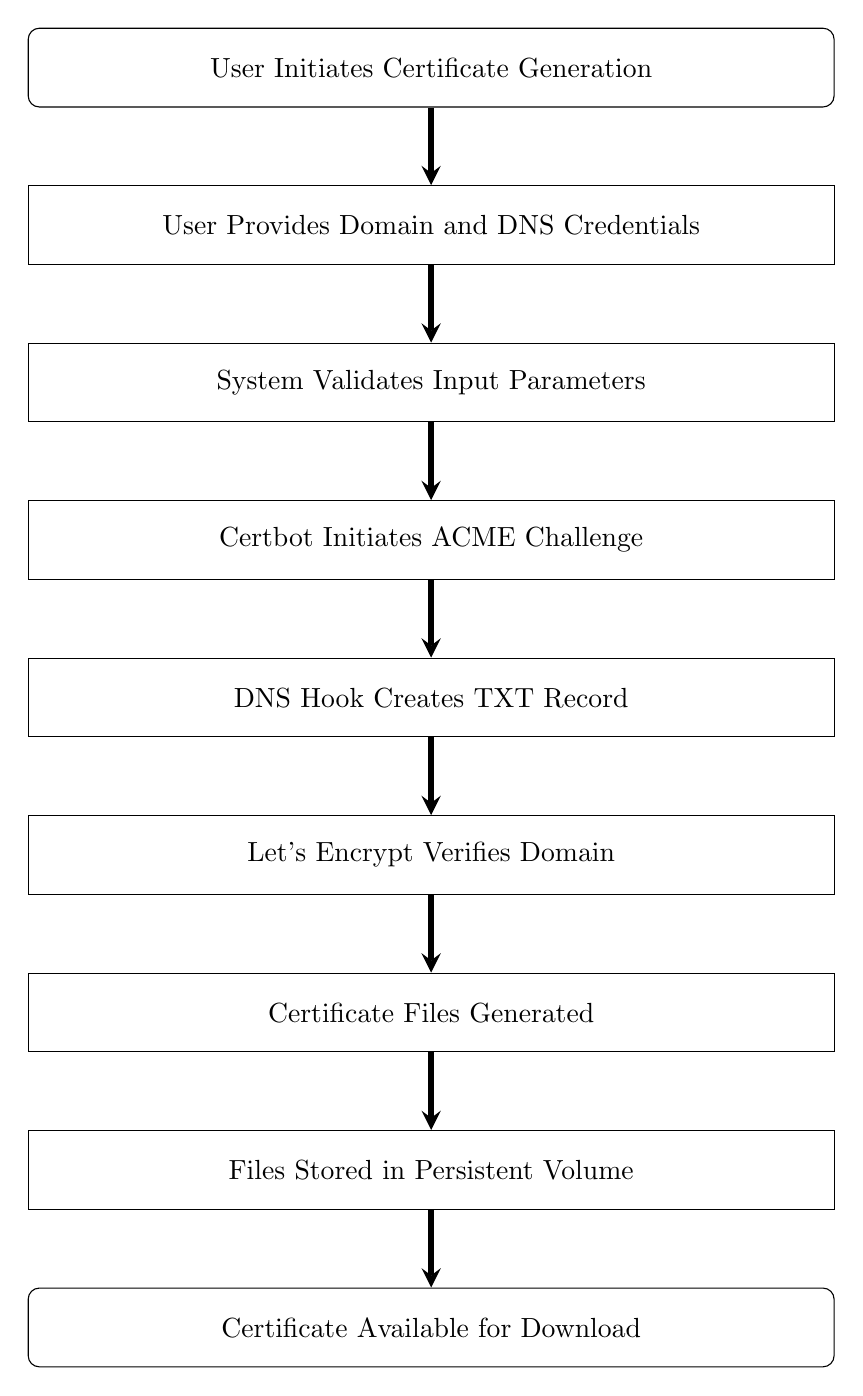
\begin{tikzpicture}[node distance=2cm]

\node (start) [startstop] {User Initiates Certificate Generation};
\node (input) [process, below of=start] {User Provides Domain and DNS Credentials};
\node (validate) [process, below of=input] {System Validates Input Parameters};
\node (certbot) [process, below of=validate] {Certbot Initiates ACME Challenge};
\node (dns) [process, below of=certbot] {DNS Hook Creates TXT Record};
\node (verify) [process, below of=dns] {Let's Encrypt Verifies Domain};
\node (generate) [process, below of=verify] {Certificate Files Generated};
\node (store) [process, below of=generate] {Files Stored in Persistent Volume};
\node (complete) [startstop, below of=store] {Certificate Available for Download};

\draw [arrow] (start) -- (input);
\draw [arrow] (input) -- (validate);
\draw [arrow] (validate) -- (certbot);
\draw [arrow] (certbot) -- (dns);
\draw [arrow] (dns) -- (verify);
\draw [arrow] (verify) -- (generate);
\draw [arrow] (generate) -- (store);
\draw [arrow] (store) -- (complete);

\end{tikzpicture}
\caption{Certificate Generation Process Flow}
\label{fig:cert-generation-flow}
\end{figure}

\subsection{Error Handling Workflow}

The system implements comprehensive error handling at each stage:

\begin{enumerate}
    \item \textbf{Input Validation Errors}: Form validation provides immediate feedback
    \item \textbf{DNS API Errors}: Credential validation and API response handling
    \item \textbf{ACME Challenge Errors}: Retry mechanisms with exponential backoff
    \item \textbf{Certificate Generation Errors}: Detailed error reporting and recovery guidance
\end{enumerate}

\subsection{System Architecture Flow}

\begin{figure}[h]
\centering
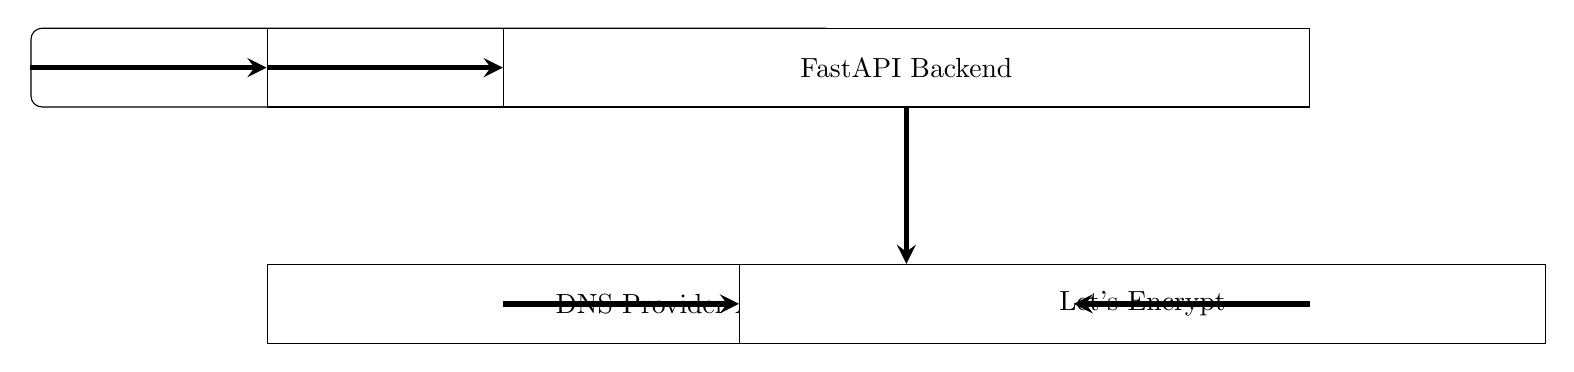
\begin{tikzpicture}[node distance=3cm]

\node (user) [startstop] {User Browser};
\node (frontend) [process, right of=user] {React Frontend};
\node (api) [process, right of=frontend] {FastAPI Backend};
\node (certbot) [process, below of=api] {Certbot Service};
\node (dns) [process, left of=certbot] {DNS Provider API};
\node (le) [process, right of=certbot] {Let's Encrypt};

\draw [arrow] (user) -- (frontend);
\draw [arrow] (frontend) -- (api);
\draw [arrow] (api) -- (certbot);
\draw [arrow] (certbot) -- (dns);
\draw [arrow] (certbot) -- (le);

\end{tikzpicture}
\caption{System Architecture Data Flow}
\label{fig:system-architecture-flow}
\end{figure}

\section{Drawbacks and Limitations}

\subsection{Current System Limitations}

\begin{enumerate}
    \item \textbf{DNS Provider Support}
    \begin{itemize}
        \item Currently limited to GoDaddy DNS provider only
        \item No support for other major providers (Cloudflare, AWS Route53, etc.)
        \item Manual configuration required for each DNS provider
    \end{itemize}
    
    \item \textbf{Authentication and Security}
    \begin{itemize}
        \item No built-in user authentication system
        \item API credentials handled client-side only
        \item No role-based access control implementation
    \end{itemize}
    
    \item \textbf{Certificate Management}
    \begin{itemize}
        \item No automatic certificate renewal scheduling
        \item No certificate revocation capabilities
        \item Limited certificate metadata tracking
    \end{itemize}
    
    \item \textbf{Scalability Constraints}
    \begin{itemize}
        \item Single-instance deployment architecture
        \item No database integration for certificate metadata
        \item Limited concurrent request handling
    \end{itemize}
\end{enumerate}

\subsection{Technical Limitations}

\begin{enumerate}
    \item \textbf{Dependency on External Services}
    \begin{itemize}
        \item Reliance on Let's Encrypt service availability
        \item DNS provider API rate limiting
        \item Internet connectivity requirements
    \end{itemize}
    
    \item \textbf{Error Recovery}
    \begin{itemize}
        \item Limited automated error recovery mechanisms
        \item Manual intervention required for complex failures
        \item No automatic retry for transient failures
    \end{itemize}
\end{enumerate}

\section{Proposed Enhancements}

\subsection{Short-term Improvements}

\begin{enumerate}
    \item \textbf{Multi-DNS Provider Support}
    \begin{itemize}
        \item Implement Cloudflare DNS integration
        \item Add AWS Route53 support
        \item Create abstract DNS provider interface
    \end{itemize}
    
    \item \textbf{Enhanced Security}
    \begin{itemize}
        \item Implement JWT-based authentication
        \item Add API key management system
        \item Implement request rate limiting
    \end{itemize}
    
    \item \textbf{Improved User Experience}
    \begin{itemize}
        \item Add certificate renewal notifications
        \item Implement bulk certificate operations
        \item Enhanced error messaging and recovery guidance
    \end{itemize}
\end{enumerate}

\subsection{Long-term Enhancements}

\begin{enumerate}
    \item \textbf{Enterprise Features}
    \begin{itemize}
        \item Multi-tenant architecture
        \item Advanced monitoring and analytics
        \item Integration with CI/CD pipelines
    \end{itemize}
    
    \item \textbf{Automation Improvements}
    \begin{itemize}
        \item Automatic certificate renewal scheduling
        \item Certificate lifecycle automation
        \item Integration with certificate deployment tools
    \end{itemize}
    
    \item \textbf{Scalability Enhancements}
    \begin{itemize}
        \item Database integration for metadata management
        \item Microservices architecture implementation
        \item Horizontal scaling capabilities
    \end{itemize}
\end{enumerate}

\section{Conclusions}

The SSL Automation Tool successfully addresses the primary challenge of automating SSL certificate generation and management through Let's Encrypt integration. The system provides:

\begin{itemize}
    \item Streamlined certificate generation with DNS-01 validation
    \item User-friendly web interface with comprehensive documentation
    \item Robust backend API with proper error handling
    \item Container-based deployment for easy scaling
    \item Extensible architecture for future enhancements
\end{itemize}

The project demonstrates effective integration of modern web technologies (React 19, Next.js 15, FastAPI) with established certificate management tools (Certbot, Let's Encrypt) to create a practical solution for SSL certificate automation.

Future development should focus on expanding DNS provider support, implementing authentication mechanisms, and adding advanced monitoring capabilities to create a comprehensive enterprise-grade certificate management platform.
  % User Manual

\clearpage % Start a new page
%----------------------------------------------------------------------------------------
%	THESIS CONTENT - APPENDICES
%----------------------------------------------------------------------------------------

\addtocontents{toc}{\vspace{2em}} % Add a gap in the Contents, for aesthetics

\appendix % Cue to tell LaTeX that the following 'chapters' are Appendices

% Include the appendices of the thesis as separate files from the Appendices folder
% Following the project report structure from the guide

% Appendix A

\chapter{User Interface Screens} % Main appendix title

\label{AppendixA} % For referencing this appendix elsewhere, use \ref{AppendixA}

% Header formatting is now handled in main.tex

This appendix contains screenshots and descriptions of the user interface screens of the SSL Automation Tool.

\section{Main Dashboard}

The SSL Certificate Dashboard serves as the central hub for certificate management operations. It provides an overview of all certificates, their status, and quick access to essential functions.

\subsection{Dashboard Overview}

The main dashboard features:
\begin{itemize}
    \item Statistics cards showing certificate counts and status
    \item Certificate list with sortable columns
    \item Quick action buttons for certificate operations
    \item Responsive design for mobile and desktop use
\end{itemize}

\subsection{Statistics Section}

The statistics cards display:
\begin{itemize}
    \item \textbf{Total Certificates}: Aggregate count of all managed certificates
    \item \textbf{Valid Certificates}: Number of currently valid certificates
    \item \textbf{Expiring Soon}: Certificates expiring within 30 days (yellow warning)
    \item \textbf{Invalid Certificates}: Expired or problematic certificates (red alert)
\end{itemize}

\section{Certificate Generation Dialog}

The certificate generation interface provides a comprehensive form for creating new SSL certificates with proper validation and user guidance.

\subsection{Basic Information Fields}

\begin{itemize}
    \item \textbf{Domain}: Target domain for certificate generation
    \item \textbf{Email}: Contact email for Let's Encrypt registration
    \item \textbf{DNS Provider}: Currently supporting GoDaddy with dropdown selection
\end{itemize}

\subsection{DNS Configuration Section}

\begin{itemize}
    \item \textbf{API Key}: Secure input field for DNS provider API key
    \item \textbf{API Secret}: Password-masked field for API secret
    \item \textbf{Base Domain}: Base domain for DNS record management
\end{itemize}

\subsection{Advanced Settings (Expandable)}

\begin{itemize}
    \item \textbf{TTL Setting}: Configurable DNS record time-to-live (default: 600)
    \item \textbf{Propagation Delay}: DNS propagation wait time (default: 60 seconds)
\end{itemize}

\subsection{Progress Indicators}

During certificate generation, the interface shows:
\begin{itemize}
    \item Real-time progress updates
    \item Step-by-step process indicators
    \item Success/error notifications
    \item Loading animations for user feedback
\end{itemize}

\section{Certificate List View}

The certificate list provides comprehensive management capabilities with sortable columns and action buttons.

\subsection{Column Information}

\begin{itemize}
    \item \textbf{Domain}: Certificate domain name with support for wildcards
    \item \textbf{Status Badge}: Color-coded status indicator
    \begin{itemize}
        \item Green: Valid certificate (>30 days remaining)
        \item Yellow: Expiring soon (7-30 days remaining)
        \item Red: Expired or invalid (<7 days or expired)
    \end{itemize}
    \item \textbf{Issued Date}: Certificate generation timestamp
    \item \textbf{Expires On}: Certificate expiration date
    \item \textbf{Actions}: Download and management options
\end{itemize}

\subsection{Action Buttons}

Each certificate row provides:
\begin{itemize}
    \item \textbf{Download Fullchain}: Downloads fullchain.pem file
    \item \textbf{Download Private Key}: Downloads privkey.pem file
    \item \textbf{Download ZIP}: Downloads complete certificate bundle
    \item \textbf{View Details}: Shows detailed certificate information
\end{itemize}

\section{Documentation Interface}

The documentation system provides comprehensive guides for server configuration and certificate deployment.

\subsection{Tab Navigation}

The documentation is organized into tabs:
\begin{itemize}
    \item \textbf{Overview}: General information about SSL certificates
    \item \textbf{Nginx}: Complete Nginx SSL configuration guide
    \item \textbf{Apache}: Apache HTTP server SSL setup
    \item \textbf{Docker}: Container-based deployment strategies
    \item \textbf{Troubleshooting}: Common issues and solutions
\end{itemize}

\subsection{Code Examples}

Each documentation section includes:
\begin{itemize}
    \item Syntax-highlighted configuration examples
    \item Copy-to-clipboard functionality
    \item Step-by-step implementation guides
    \item Best practices and security recommendations
\end{itemize}

\section{Dark Mode Interface}

The application supports both light and dark themes with automatic detection and manual toggle capabilities.

\subsection{Theme Features}

\begin{itemize}
    \item \textbf{Automatic Detection}: Respects system theme preferences
    \item \textbf{Manual Toggle}: Theme switcher in the header
    \item \textbf{Consistent Styling}: All components adapt to theme changes
    \item \textbf{Accessibility}: High contrast ratios for readability
\end{itemize}

\section{Mobile Responsive Design}

The interface adapts to various screen sizes and device orientations.

\subsection{Mobile Adaptations}

\begin{itemize}
    \item \textbf{Responsive Grid}: Statistics cards stack vertically on mobile
    \item \textbf{Collapsible Tables}: Certificate list optimized for mobile viewing
    \item \textbf{Touch-Friendly}: Buttons and interactions optimized for touch
    \item \textbf{Navigation}: Hamburger menu for mobile navigation
\end{itemize}

\subsection{Tablet Interface}

\begin{itemize}
    \item \textbf{Hybrid Layout}: Combines desktop and mobile elements
    \item \textbf{Split View}: Side-by-side content where appropriate
    \item \textbf{Touch Navigation}: Optimized for tablet interaction patterns
\end{itemize}

\section{Error and Success Notifications}

The application provides comprehensive feedback through toast notifications and inline messaging.

\subsection{Notification Types}

\begin{itemize}
    \item \textbf{Success Notifications}: Green toast for successful operations
    \item \textbf{Error Messages}: Red toast with detailed error information
    \item \textbf{Warning Alerts}: Yellow notifications for important information
    \item \textbf{Info Messages}: Blue notifications for general information
\end{itemize}

\subsection{Error Handling Interface}

\begin{itemize}
    \item \textbf{Form Validation}: Real-time field validation with error highlighting
    \item \textbf{API Error Display}: Detailed error messages from backend operations
    \item \textbf{Retry Mechanisms}: Options to retry failed operations
    \item \textbf{Help Context}: Links to relevant documentation for error resolution
\end{itemize}

 % User Interface Screens
% Appendix B

\chapter{Sample Program Code} % Main appendix title

\label{AppendixB} % For referencing this appendix elsewhere, use \ref{AppendixB}

% Header formatting is now handled in main.tex

This appendix contains key program code samples that demonstrate the core functionality and implementation details of the SSL Automation Tool.

\section{Frontend Code Samples}

\subsection{SSL Dashboard Component}

The main dashboard component that manages certificate display and operations:

\begin{verbatim}
// SSLDashboard.tsx - Main certificate management interface
import React, { useState, useEffect } from 'react';
import { Card, CardContent, CardHeader, CardTitle } from '@/components/ui/card';
import { Button } from '@/components/ui/button';
import { SSLApiService } from '@/lib/api';
import { Certificate } from '@/types/ssl';

export function SSLDashboard() {
  const [certificates, setCertificates] = useState<Certificate[]>([]);
  const [loading, setLoading] = useState(true);

  useEffect(() => {
    loadCertificates();
  }, []);

  const loadCertificates = async () => {
    try {
      setLoading(true);
      const response = await SSLApiService.listCertificates();
      setCertificates(response.certificates);
    } catch (error) {
      console.error('Failed to load certificates:', error);
    } finally {
      setLoading(false);
    }
  };

  const downloadCertificate = async (domain: string, type: string) => {
    try {
      const blob = await SSLApiService.downloadCertificateFile(domain, type);
      SSLApiService.triggerDownload(blob, `${domain}-${type}.pem`);
    } catch (error) {
      console.error('Download failed:', error);
    }
  };

  const getStatusColor = (cert: Certificate) => {
    if (!cert.valid) return 'red';
    const daysUntilExpiry = Math.ceil(
      (new Date(cert.expires_on).getTime() - Date.now()) / (1000 * 60 * 60 * 24)
    );
    if (daysUntilExpiry < 7) return 'red';
    if (daysUntilExpiry < 30) return 'yellow';
    return 'green';
  };

  return (
    <div className="space-y-6">
      <div className="grid grid-cols-1 md:grid-cols-4 gap-4">
        {/* Statistics Cards */}
        <Card>
          <CardHeader>
            <CardTitle>Total Certificates</CardTitle>
          </CardHeader>
          <CardContent>
            <div className="text-2xl font-bold">{certificates.length}</div>
          </CardContent>
        </Card>
        {/* Additional statistics cards... */}
      </div>
      
      {/* Certificate List */}
      <Card>
        <CardHeader>
          <CardTitle>Certificate Management</CardTitle>
        </CardHeader>
        <CardContent>
          {certificates.map((cert) => (
            <div key={cert.domain} className="border-b py-4">
              <div className="flex justify-between items-center">
                <div>
                  <h3 className="font-medium">{cert.domain}</h3>
                  <p className="text-sm text-gray-500">
                    Expires: {new Date(cert.expires_on).toLocaleDateString()}
                  </p>
                </div>
                <div className="flex space-x-2">
                  <Button
                    onClick={() => downloadCertificate(cert.domain, 'fullchain')}
                    size="sm"
                  >
                    Download Fullchain
                  </Button>
                  <Button
                    onClick={() => downloadCertificate(cert.domain, 'privkey')}
                    size="sm"
                  >
                    Download Private Key
                  </Button>
                </div>
              </div>
            </div>
          ))}
        </CardContent>
      </Card>
    </div>
  );
}
\end{verbatim}

\subsection{Certificate Generation Form}

Form component for creating new SSL certificates:

\begin{verbatim}
// CertificateGenerationDialog.tsx - Certificate creation interface
import React from 'react';
import { useForm } from 'react-hook-form';
import { zodResolver } from '@hookform/resolvers/zod';
import * as z from 'zod';
import { Button } from '@/components/ui/button';
import { Input } from '@/components/ui/input';
import { Label } from '@/components/ui/label';
import { SSLApiService } from '@/lib/api';

const formSchema = z.object({
  domain: z.string().min(1, 'Domain is required'),
  email: z.string().email('Valid email is required'),
  dns_provider: z.literal('godaddy'),
  api_key: z.string().min(1, 'API key is required'),
  api_secret: z.string().min(1, 'API secret is required'),
  base_domain: z.string().min(1, 'Base domain is required'),
  ttl: z.number().min(300).max(86400).optional(),
  propagation_delay: z.number().min(30).max(600).optional(),
});

type FormData = z.infer<typeof formSchema>;

export function CertificateGenerationDialog({ onSuccess, onClose }) {
  const [isGenerating, setIsGenerating] = useState(false);
  
  const form = useForm<FormData>({
    resolver: zodResolver(formSchema),
    defaultValues: {
      dns_provider: 'godaddy',
      ttl: 600,
      propagation_delay: 60,
    },
  });

  const onSubmit = async (data: FormData) => {
    try {
      setIsGenerating(true);
      const response = await SSLApiService.generateCertificate(data);
      
      if (response.success) {
        toast.success('Certificate generated successfully!');
        onSuccess();
        onClose();
      } else {
        toast.error(`Generation failed: ${response.error}`);
      }
    } catch (error) {
      toast.error('Failed to generate certificate');
      console.error(error);
    } finally {
      setIsGenerating(false);
    }
  };

  return (
    <form onSubmit={form.handleSubmit(onSubmit)} className="space-y-4">
      <div>
        <Label htmlFor="domain">Domain</Label>
        <Input
          id="domain"
          placeholder="example.com or *.example.com"
          {...form.register('domain')}
        />
        {form.formState.errors.domain && (
          <p className="text-red-500 text-sm">
            {form.formState.errors.domain.message}
          </p>
        )}
      </div>

      <div>
        <Label htmlFor="email">Email</Label>
        <Input
          id="email"
          type="email"
          placeholder="admin@example.com"
          {...form.register('email')}
        />
      </div>

      <div>
        <Label htmlFor="api_key">GoDaddy API Key</Label>
        <Input
          id="api_key"
          type="password"
          {...form.register('api_key')}
        />
      </div>

      <div>
        <Label htmlFor="api_secret">GoDaddy API Secret</Label>
        <Input
          id="api_secret"
          type="password"
          {...form.register('api_secret')}
        />
      </div>

      <Button 
        type="submit" 
        disabled={isGenerating}
        className="w-full"
      >
        {isGenerating ? 'Generating...' : 'Generate Certificate'}
      </Button>
    </form>
  );
}
\end{verbatim}

\section{Backend Code Samples}

\subsection{FastAPI Main Application}

The core FastAPI application setup with CORS and routing:

\begin{verbatim}
# app/main.py - FastAPI application entry point
from fastapi import FastAPI
from fastapi.middleware.cors import CORSMiddleware
from app.routes import certs

app = FastAPI(
    title="SSL Automation API",
    description="Automated SSL certificate generation using Let's Encrypt",
    version="1.0.0"
)

# CORS configuration for frontend integration
app.add_middleware(
    CORSMiddleware,
    allow_origins=[
        "http://localhost:3000",
        "http://localhost:3001",
        "http://127.0.0.1:3000",
        "http://127.0.0.1:3001"
    ],
    allow_credentials=True,
    allow_methods=["*"],
    allow_headers=["*"],
)

# Include certificate management routes
app.include_router(certs.router, prefix="/api/v1")

@app.get("/")
async def root():
    return {"message": "SSL Automation API is running"}

@app.get("/health")
async def health_check():
    return {"status": "healthy", "service": "ssl-automation-api"}
\end{verbatim}

\subsection{Certificate Service Implementation}

Core business logic for certificate operations:

\begin{verbatim}
# app/services/cert_service.py - Certificate file operations
import os
import zipfile
from pathlib import Path
from typing import Optional, Dict, List
from app.utils.cert_info import get_cert_info

class CertService:
    @staticmethod
    def get_cert_paths(domain: str) -> Optional[Dict[str, str]]:
        """Get paths to certificate files for a domain."""
        cert_dir = Path(f"/etc/letsencrypt/live/{domain}")
        
        if not cert_dir.exists():
            return None
            
        fullchain_path = cert_dir / "fullchain.pem"
        privkey_path = cert_dir / "privkey.pem"
        
        if fullchain_path.exists() and privkey_path.exists():
            return {
                "fullchain": str(fullchain_path),
                "privkey": str(privkey_path)
            }
        
        return None
    
    @staticmethod
    def create_cert_zip(domain: str) -> Optional[str]:
        """Create a ZIP archive containing all certificate files."""
        cert_paths = CertService.get_cert_paths(domain)
        if not cert_paths:
            return None
            
        zip_path = f"/tmp/{domain}-certificates.zip"
        
        with zipfile.ZipFile(zip_path, 'w') as zipf:
            for file_type, file_path in cert_paths.items():
                if os.path.exists(file_path):
                    zipf.write(file_path, f"{file_type}.pem")
        
        return zip_path if os.path.exists(zip_path) else None
    
    @staticmethod
    def list_all_certificates() -> List[Dict]:
        """List all managed certificates with their information."""
        certificates = []
        le_dir = Path("/etc/letsencrypt/live")
        
        if not le_dir.exists():
            return certificates
            
        for domain_dir in le_dir.iterdir():
            if domain_dir.is_dir():
                cert_info = get_cert_info(domain_dir.name)
                if cert_info:
                    certificates.append(cert_info)
                    
        return certificates
\end{verbatim}

\subsection{Certbot Runner Service}

Service for executing Certbot commands with DNS validation:

\begin{verbatim}
# app/services/certbot_runner.py - Certbot execution wrapper
import subprocess
import os
import logging
from typing import Dict, Tuple

logger = logging.getLogger(__name__)

class CertbotRunner:
    @staticmethod
    def generate_certificate(
        domain: str,
        email: str,
        dns_provider: str,
        api_key: str,
        api_secret: str,
        base_domain: str,
        ttl: int = 600,
        propagation_delay: int = 60
    ) -> Tuple[bool, str]:
        """Execute Certbot to generate SSL certificate."""
        
        # Set environment variables for DNS hook
        env = os.environ.copy()
        env.update({
            'GODADDY_API_KEY': api_key,
            'GODADDY_API_SECRET': api_secret,
            'BASE_DOMAIN': base_domain,
            'DNS_TTL': str(ttl),
            'PROPAGATION_DELAY': str(propagation_delay)
        })
        
        # Construct Certbot command
        cmd = [
            'certbot', 'certonly',
            '--manual',
            '--preferred-challenges=dns',
            '--manual-auth-hook', '/app/scripts/godaddy_auth_hook.py',
            '--manual-cleanup-hook', '/app/scripts/godaddy_cleanup_hook.py',
            '--domain', domain,
            '--email', email,
            '--agree-tos',
            '--non-interactive',
            '--manual-public-ip-logging-ok'
        ]
        
        try:
            logger.info(f"Starting certificate generation for {domain}")
            
            result = subprocess.run(
                cmd,
                env=env,
                capture_output=True,
                text=True,
                timeout=300  # 5 minute timeout
            )
            
            if result.returncode == 0:
                logger.info(f"Certificate generated successfully for {domain}")
                return True, result.stdout
            else:
                logger.error(f"Certbot failed for {domain}: {result.stderr}")
                return False, result.stderr
                
        except subprocess.TimeoutExpired:
            logger.error(f"Certbot timeout for {domain}")
            return False, "Certificate generation timed out"
        except Exception as e:
            logger.error(f"Certbot execution failed for {domain}: {str(e)}")
            return False, f"Execution failed: {str(e)}"
\end{verbatim}

\section{DNS Integration Code}

\subsection{GoDaddy DNS Hook Script}

Python script for automated DNS challenge handling:

\begin{verbatim}
#!/usr/bin/env python3
# app/scripts/godaddy_auth_hook.py - GoDaddy DNS authentication hook

import os
import sys
import requests
import time
import logging

logging.basicConfig(level=logging.INFO)
logger = logging.getLogger(__name__)

def create_txt_record():
    """Create TXT record for DNS challenge validation."""
    
    # Get environment variables set by Certbot
    domain = os.environ.get('CERTBOT_DOMAIN')
    validation = os.environ.get('CERTBOT_VALIDATION')
    
    # Get GoDaddy API credentials
    api_key = os.environ.get('GODADDY_API_KEY')
    api_secret = os.environ.get('GODADDY_API_SECRET')
    base_domain = os.environ.get('BASE_DOMAIN')
    ttl = int(os.environ.get('DNS_TTL', 600))
    delay = int(os.environ.get('PROPAGATION_DELAY', 60))
    
    if not all([domain, validation, api_key, api_secret, base_domain]):
        logger.error("Missing required environment variables")
        sys.exit(1)
    
    # Construct record name
    record_name = f"_acme-challenge.{domain}"
    if domain.startswith('*.'):
        record_name = f"_acme-challenge.{domain[2:]}"
    
    # Remove base domain from record name for GoDaddy API
    if record_name.endswith(f".{base_domain}"):
        record_name = record_name[:-len(f".{base_domain}")]
    
    # GoDaddy API headers
    headers = {
        'Authorization': f'sso-key {api_key}:{api_secret}',
        'Content-Type': 'application/json'
    }
    
    # Record data
    record_data = [{
        'data': validation,
        'ttl': ttl
    }]
    
    # API endpoint
    url = f"https://api.godaddy.com/v1/domains/{base_domain}/records/TXT/{record_name}"
    
    try:
        logger.info(f"Creating TXT record: {record_name} = {validation}")
        
        response = requests.put(url, json=record_data, headers=headers)
        response.raise_for_status()
        
        logger.info(f"TXT record created successfully")
        logger.info(f"Waiting {delay} seconds for DNS propagation...")
        
        time.sleep(delay)
        
        logger.info("DNS propagation wait complete")
        
    except requests.exceptions.RequestException as e:
        logger.error(f"Failed to create TXT record: {e}")
        sys.exit(1)

if __name__ == "__main__":
    create_txt_record()
\end{verbatim}

\section{API Models and Types}

\subsection{Pydantic Models}

Data validation models for API requests and responses:

\begin{verbatim}
# app/models/models.py - Pydantic data models
from pydantic import BaseModel, EmailStr
from typing import Optional, List
from datetime import datetime

class CertRequest(BaseModel):
    """Certificate generation request model."""
    domain: str
    email: EmailStr
    dns_provider: str = "godaddy"
    api_key: str
    api_secret: str
    base_domain: str
    ttl: Optional[int] = 600
    propagation_delay: Optional[int] = 60

class CertFetchRequest(BaseModel):
    """Certificate retrieval request model."""
    domain: str

class Certificate(BaseModel):
    """Certificate information model."""
    domain: str
    issued_on: str
    expires_on: str
    valid: bool
    fullchain_path: Optional[str] = None
    privkey_path: Optional[str] = None

class CertificateListResponse(BaseModel):
    """Certificate list response model."""
    certificates: List[Certificate]
    total: int

class CertificateGenerationResponse(BaseModel):
    """Certificate generation response model."""
    success: bool
    message: str
    domain: Optional[str] = None
    error: Optional[str] = None
    output: Optional[str] = None
\end{verbatim}

\section{Configuration Files}

\subsection{Docker Configuration}

Docker Compose setup for containerized deployment:

\begin{verbatim}
# docker-compose.yml - Container orchestration
version: '3.8'

services:
  ssl-automation-backend:
    build: .
    ports:
      - "80:8000"
    volumes:
      - .:/app
      - cert-data:/etc/letsencrypt
    environment:
      - PYTHONPATH=/app
    working_dir: /app
    command: uv run uvicorn app.main:app --host 0.0.0.0 --port 8000

volumes:
  cert-data:
    driver: local
\end{verbatim}

\subsection{Python Project Configuration}

Modern Python project setup with UV package manager:

\begin{verbatim}
# pyproject.toml - Python project configuration
[project]
name = "ssl-automation-backend"
version = "0.1.0"
description = "Automated SSL certificate generation using Let's Encrypt"
readme = "README.md"
requires-python = ">=3.13"

dependencies = [
    "fastapi>=0.115.12",
    "uvicorn>=0.34.3",
    "pydantic>=2.5.0",
    "pydantic[email]>=2.5.0",
    "certbot>=4.1.1",
    "cryptography>=45.0.4",
    "requests>=2.31.0",
    "python-multipart>=0.0.6"
]

[build-system]
requires = ["hatchling"]
build-backend = "hatchling.build"

[tool.uv]
dev-dependencies = [
    "pytest>=7.0.0",
    "pytest-asyncio>=0.21.0",
    "httpx>=0.24.0"
]
\end{verbatim}

 % Sample Program Code
% Appendix C

\chapter{Additional Documentation} % Main appendix title

\label{AppendixC} % For referencing this appendix elsewhere, use \ref{AppendixC}

% Header formatting is now handled in main.tex

This appendix contains additional technical documentation, API references, and deployment guides that support the SSL Automation Tool implementation.

\section{API Documentation}

\subsection{REST API Endpoints}

The SSL Automation Tool provides a comprehensive REST API for certificate management operations.

\subsubsection{Certificate Generation}

\textbf{Endpoint}: \texttt{POST /api/v1/generate-cert}

\textbf{Description}: Initiates SSL certificate generation using Let's Encrypt with DNS validation.

\textbf{Request Body}:
\begin{verbatim}
{
  "domain": "example.com",
  "email": "admin@example.com",
  "dns_provider": "godaddy",
  "api_key": "your_godaddy_api_key",
  "api_secret": "your_godaddy_api_secret",
  "base_domain": "example.com",
  "ttl": 600,
  "propagation_delay": 60
}
\end{verbatim}

\textbf{Response}:
\begin{verbatim}
{
  "success": true,
  "message": "Certificate generated successfully",
  "domain": "example.com",
  "output": "Certbot execution output..."
}
\end{verbatim}

\section{Environment Configuration}

\subsection{Required Environment Variables}

The following environment variables must be configured for proper system operation:

\subsubsection{Frontend Configuration}

\begin{verbatim}
# .env.local - Frontend environment variables
NEXT_PUBLIC_API_URL=http://localhost:80
NEXT_PUBLIC_ENV=development
\end{verbatim}

\subsubsection{Backend Configuration}

Environment variables are passed at runtime through Docker or system configuration:

\begin{verbatim}
# Runtime environment variables
GODADDY_API_KEY=your_api_key_here
GODADDY_API_SECRET=your_api_secret_here
BASE_DOMAIN=yourdomain.com
DNS_TTL=600
PROPAGATION_DELAY=60
PYTHONPATH=/app
\end{verbatim}

\section{Security Considerations}

\subsection{Security Best Practices}

\subsubsection{Credential Management}

\begin{itemize}
    \item Never store DNS provider credentials in configuration files
    \item Use environment variables or secrets management systems
    \item Rotate API keys regularly (quarterly recommended)
    \item Monitor API key usage for unauthorized access
    \item Implement IP whitelisting where possible
\end{itemize}

\subsubsection{Certificate Security}

\begin{itemize}
    \item Set proper file permissions (600) for private keys
    \item Use encrypted storage for certificate backups
    \item Implement certificate pinning for critical applications
    \item Monitor certificate expiration proactively
    \item Have emergency certificate renewal procedures
\end{itemize}

 % Additional Documentation

\addtocontents{toc}{\vspace{2em}} % Add a gap in the Contents, for aesthetics

\backmatter

%----------------------------------------------------------------------------------------
%	BIBLIOGRAPHY
%----------------------------------------------------------------------------------------

\label{References}

\chead{\emph{References}} % Change the page header to say "Bibliography"
%\usepackage{natbib}
%\renewcommand{\refname}{References}

\makeatletter
\interlinepenalty=10000     % don't split a single reference across page break

\renewcommand\bibname{References}
\bibliographystyle{ieeetr} % Use the "custom" BibTeX style for formatting the Bibliography
%\setcitestyle{authoryear,open={((},close={))}}

\bibliography{references} % The references (bibliography) information are stored in the file named "Bibliography.bib"

% \newcites{publ}{Publications by the candidate}

\clearpage
\section*{Publications and Presentations}
\begin{enumerate}
    \item SSL Automation Tool Development: Presented at StartMySafari Innovations Private Limited internal technical review, June 2025.
    \item "Automated SSL Certificate Management using Let's Encrypt and DNS Validation" - Technical report submitted as part of MCA project requirements, Dr. Babasaheb Ambedkar Marathwada University, June 2025.
\end{enumerate}

\makeatother
% \newpage
% \include{LOP}
% \newpage
% \include{Biography}
% Acknowledgements

\addtocontents{toc}{} % Add a gap in the Contents, for aesthetics
\thispagestyle{empty}
\acknowledgements{

I would like to express my sincere gratitude to all those who contributed to the successful completion of this SSL Automation Tool project.

First and foremost, I extend my heartfelt thanks to \textbf{Dr. Kavari Lad}, my project guide, for his invaluable guidance, continuous support, and expert advice throughout the development of this project. His insights into modern web technologies and security practices were instrumental in shaping this work.

I am deeply grateful to \textbf{StartMySafari Innovations Private Limited (smsipl)} for providing the opportunity to work on this practical and industry-relevant project. The real-world exposure and access to modern development tools and technologies significantly enhanced my learning experience.

Special thanks to \textbf{Prof. Abhijeet Shelke}, Director, for his administrative support and for creating an environment conducive to learning and innovation.

I would like to acknowledge the faculty members of the Department of Management Science at \textbf{Dr. Babasaheb Ambedkar Marathwada University, Chhatrapati Sambhajinagar}, for their academic support and for providing the foundational knowledge that enabled me to undertake this project.

My appreciation extends to the open-source community, particularly the developers of React, Next.js, FastAPI, and Let's Encrypt, whose technologies formed the backbone of this SSL automation solution.

I am thankful to my colleagues and peers who provided feedback and suggestions during the development and testing phases of the project.

Finally, I express my gratitude to my family and friends for their constant encouragement and support throughout my academic journey.

This project has been an enriching experience that has significantly enhanced my understanding of web development, SSL certificate management, and modern software engineering practices.

\begin{flushleft}
    \textbf{\authornames}\\
    June 2025
\end{flushleft}
}
% 

% Command for setting the heading on chapter pages to plain style
\let\origchapter\chapter
\renewcommand{\chapter}[1]{%
  \origchapter{#1}%
  \thispagestyle{plain}% Use plain style for the first page of each chapter
}

% Add 2 blank pages at the end of the document
\thispagestyle{empty}
\null
\newpage

\thispagestyle{empty}
\null
\newpage

\end{document}  
